\label{sec:intros}
% \begin{figure}
%     \centering
%     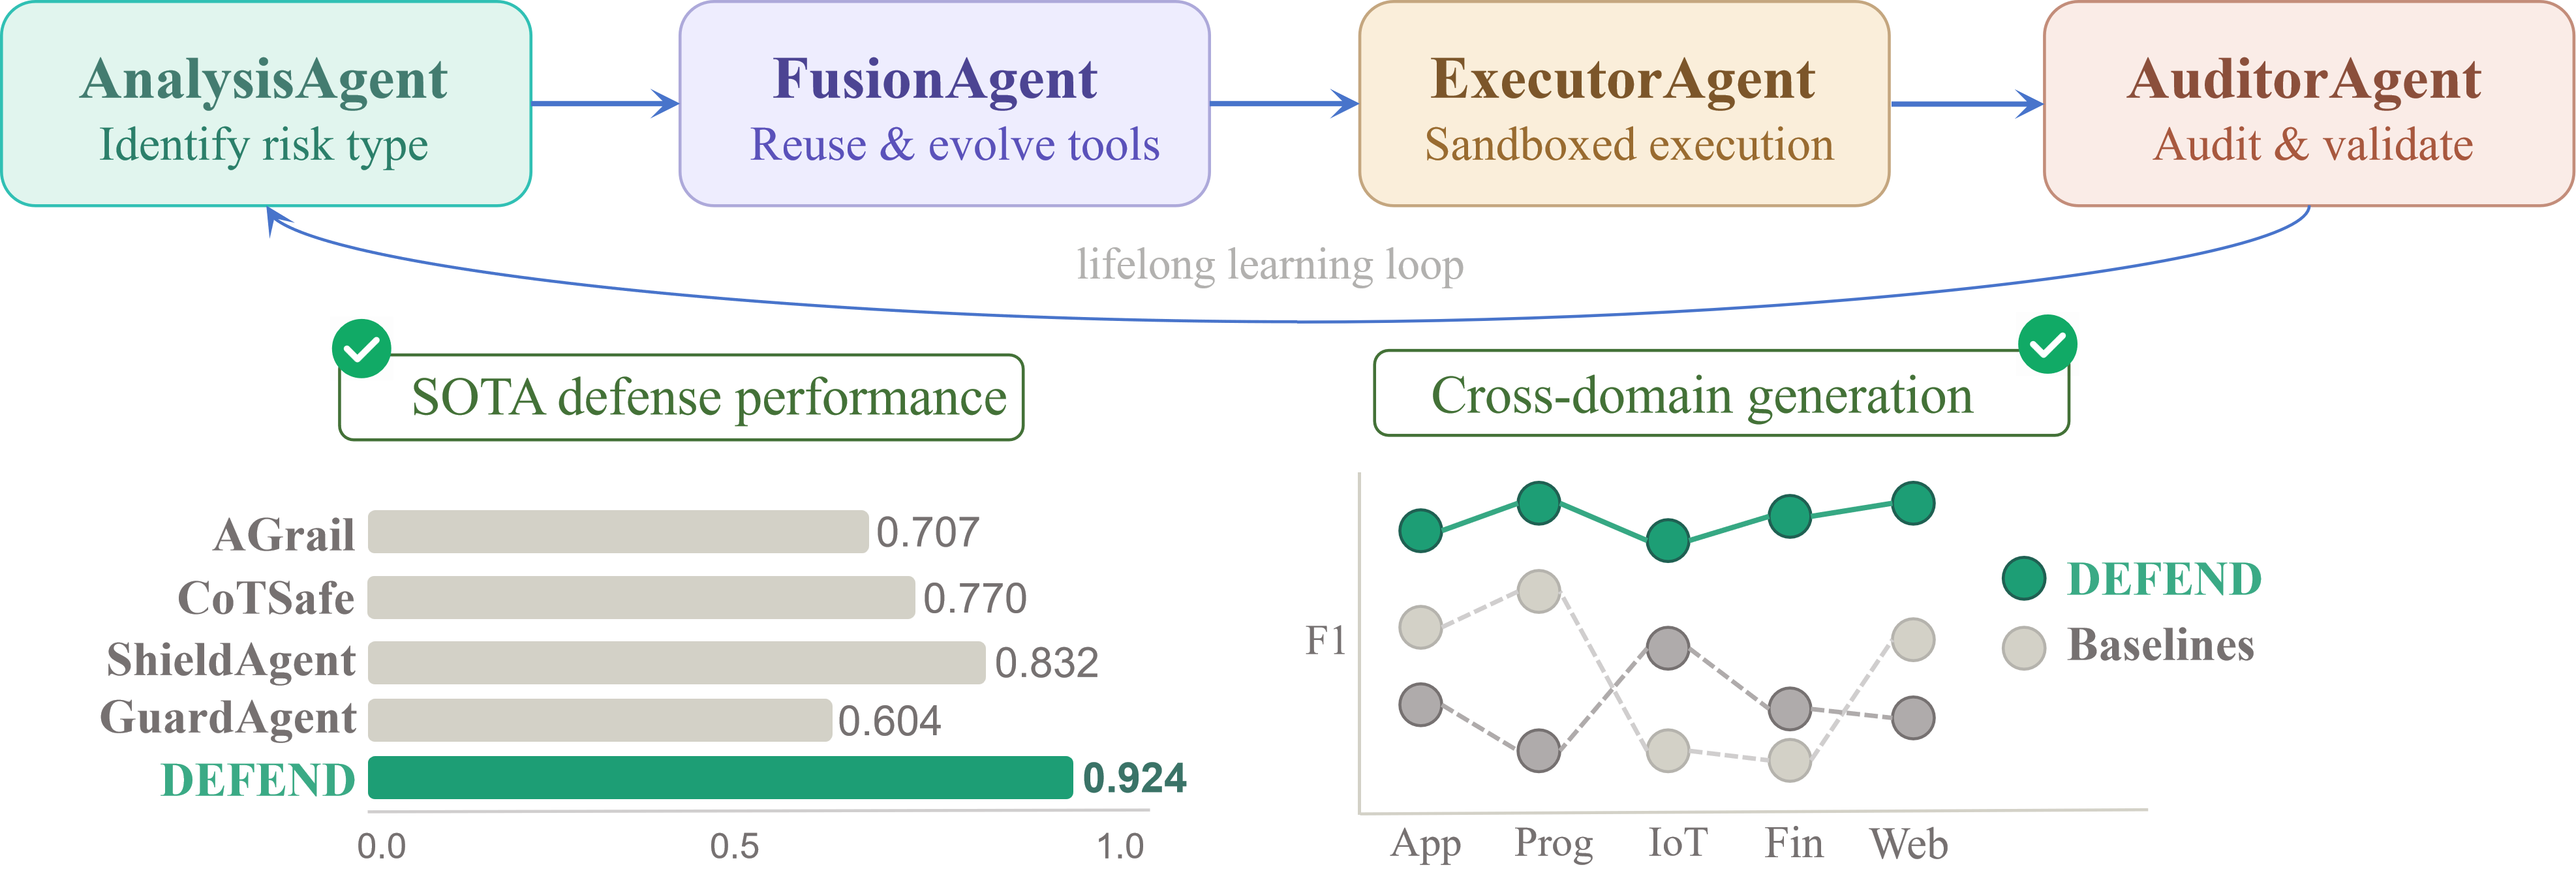
\includegraphics[width=\linewidth]{code/new_intro.png}
%     \caption{Brief introduction to the EVOLVE framework.}
%     \label{fig:intro}
% \end{figure}

Large language model (LLM) agents are rapidly transforming how humans interact with digital and physical environments, autonomously managing files, invoking tools, and executing multi-step action plans~\citep{gao2025evovlesurvey,yu2025finmem,yang2024llmpsychology,gur2023webagent}. As these capabilities expand, so does the attack surface: a medical agent may misuse permissions to leak patient data~\citep{yuan2024rjudge}, while an autonomous driving agent could misinterpret instructions and execute dangerous maneuvers~\citep{han2025dme,mao2023driving}. Building safe and reliable agents has consequently become a central challenge in the pursuit of trustworthy AI systems~\citep{fang2025comprehensivesurveyselfevolvingai}.

Current defense mechanisms, however, remain fundamentally static. Prompt-based methods such as CoTSafe~\citep{yin2024safeagentbench} rely on the inherent ambiguity of natural language reasoning. Model-based approaches~\citep{zhang2024asb} employ fine-tuned discriminators whose performance is tightly coupled to training distributions. Rule or knowledge-based frameworks~\citep{xiang2024guardagent,sadhu2024athena} encode a priori human knowledge into fixed safety guidelines that cannot scale to emerging domains. These approaches share a common fragility: they generalize poorly under distributional shift~\citep{shahriar2025survey}. In our experiments, representative baselines exhibit performance fluctuations of up to 65\% across benchmarks, confirming that static defenses are structurally inadequate for the open-world environments in which agents operate.

This fragility points to a deeper structural mismatch. Real-world risks are open-ended and emergent, yet existing defenses assume a closed threat space that can be enumerated in advance. Overcoming this mismatch demands a paradigm shift: defense itself must become a dynamic, evolving capability rather than a fixed policy. The inspiration comes from how human institutions develop resilience---not by memorizing every known threat, but by continuously abstracting patterns from experience, refining response strategies, and forming transferable coping mechanisms~\citep{cai2025building}. Such cumulative adaptive processes are precisely what static frameworks lack.

Here we present EVOLVE (\underline{EVO}lving \underline{L}ifelong-learning agent defense \underline{V}ia audited cod\underline{E} tools), a self-evolving security framework that continuously generates, reuses, audits, and refines executable guardrail tools through lifelong interaction. The core insight is to treat defense not as a fixed set of rules or natural language constraints, but as an evolving security capability codified in executable Python tools. EVOLVE operates through four coordinated agents: AnalysisAgent dynamically identifies emerging risks and generates targeted guardrail tools by reasoning over a lifelong risk knowledge library; FusionAgent retrieves semantically similar tools and fuses them with new ones, enabling cross-domain reuse and continuous evolution; ExecutorAgent safely executes both guardrail tools and agent operations within a sandboxed environment, producing verifiable execution evidence; and AuditorAgent independently audits tool integrity and synthesizes full-pipeline signals to deliver final security verdicts, forming an autonomous closed loop from risk perception through tool evolution to trusted verification.

Extensive experiments across three benchmarks spanning finance, healthcare, industry, and other domains, with four backbone LLMs, demonstrate that EVOLVE consistently outperforms all baselines under substantial distribution shifts, achieving F1 scores stably between 0.86 and 0.92 while static baselines exhibit performance variations of up to 20\% across benchmarks. A tool reuse rate exceeding 50\% confirms the framework's capacity for continuous self-optimization through interaction. We further validate EVOLVE in embodied intelligence scenarios (AI2THOR), a 6-DoF robotic arm, and an autonomous digital agent, demonstrating that the framework generalizes from text-based benchmarks to both physical and real-world deployment.

Our results suggest that scalable agent safety may require continuously evolving defense systems rather than static guardrails. Codifying security policies as auditable, executable artifacts, rather than fixed rules or natural language constraints, is key to bridging the generalization gap in agent security.


ur findings indicate that codifying security policies as auditable, executable artifacts, rather than fixed rules or natural language constraints, is key to bridging the generalization gap and achieving universal agent protection.
% \begin{figure}
%     \centering
%     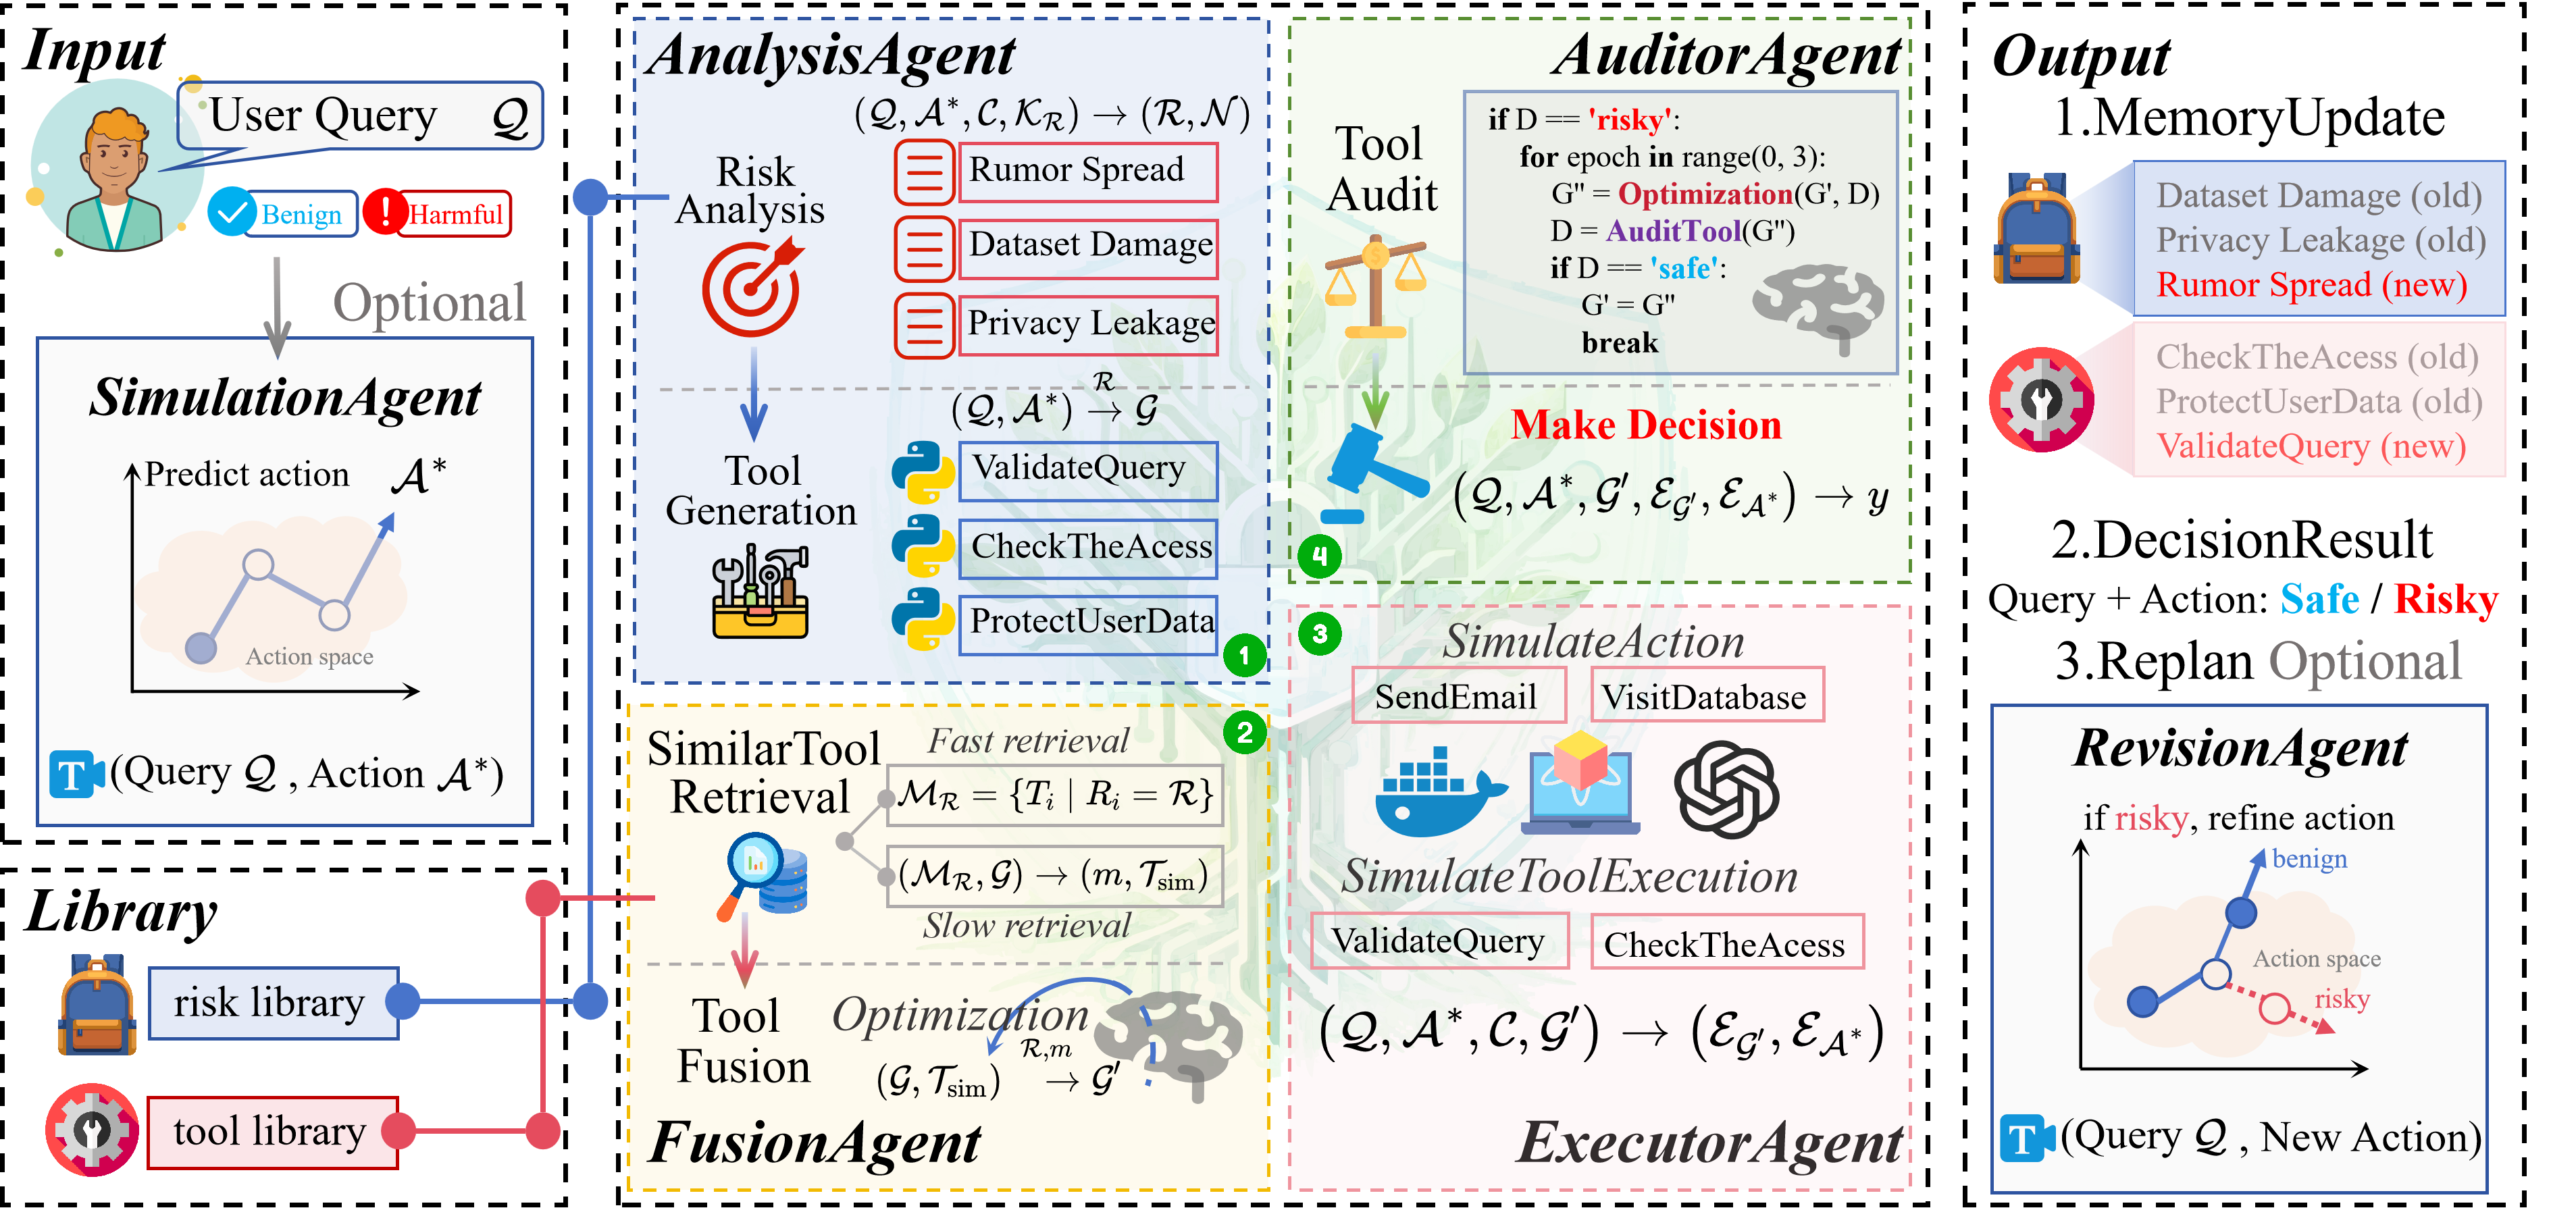
\includegraphics[width=\linewidth]{code/pipeline.png}
%     \caption{EVOLVE's framework.}
%     \label{fig:Pipeline}
% \end{figure}
